% ex: ts=2 sw=2 sts=2 et filetype=tex
% SPDX-License-Identifier: CC-BY-SA-4.0

\documentclass{article}
\usepackage[utf8]{inputenc}
\usepackage{geometry}
 \geometry{letterpaper}
 \usepackage{graphicx}
 \usepackage{titling}

 \title{Serendipia}
\author{Yolanda Alejo Huerta}
\date{Septiembre 2025}
 
 \usepackage{fancyhdr}
\fancypagestyle{plain}{%  the preset of fancyhdr 
    \fancyhf{} % clear all header and footer fields
    \fancyfoot[R]{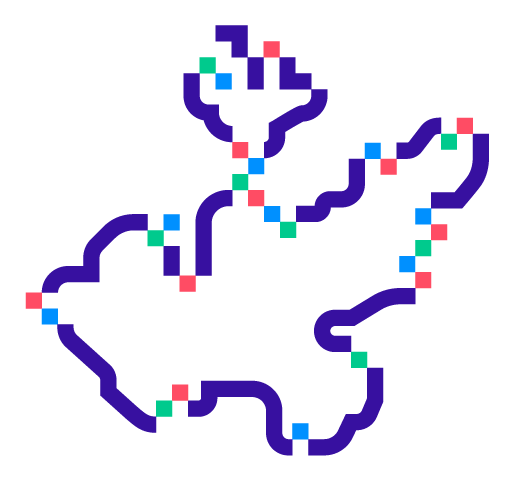
\includegraphics[width=2cm]{tsj_jalisco.png}}
    \fancyfoot[L]{\thedate}
    \fancyhead[L]{Serendipia}
    \fancyhead[R]{\theauthor}
}
\makeatletter
\def\@maketitle{%
  \newpage
  \null
  \vskip 1em%
  \begin{center}%
  \let \footnote \thanks
    {\LARGE \@title \par}%
    \vskip 1em%
    %{\large \@date}%
  \end{center}%
  \par
  \vskip 1em}
\makeatother

\usepackage{lipsum}  
\usepackage{cmbright}

\begin{document}

\maketitle

\noindent\begin{tabular}{@{}ll}
	Alumna & \theauthor\\
	Profesor & Dr. Paulo Lopez Meyer
\end{tabular}

\section*{Descripción General}

Las \textbf{ciencias exactas} (o formales) y las \textbf{ciencias sociales}
se distinguen por su objeto de estudio y, en consecuencia, por la forma en
que aplican el método científico.

\section*{Ciencias Exactas}

Las ciencias exactas son aquellas que se basan en el razonamiento
lógico-matemático para estudiar \textbf{fenómenos abstractos y
universales}. No se enfocan en hechos tangibles del mundo físico,
sino en estructuras, patrones y sistemas de pensamiento. Un ejemplo
clásico son las matemáticas y la lógica. 

\begin{itemize}
  \item \textbf{Método científico}: En estas ciencias, el método se basa
    en la \textbf{deducción} y la \textbf{demostración}. A diferencia de
    las ciencias fácticas, no se usa la experimentación para probar
    una hipótesis, sino la lógica. 
  \item \textbf{Ejemplo (Matemáticas)}: Un matemático quiere probar que
    la suma de los ángulos internos de un triángulo siempre es 180°.
    \begin{enumerate}
      \item \textbf{Formulación del problema}: ¿Es la suma de los
        ángulos internos de un triángulo siempre 180°?
      \item \textbf{Hipótesis}: La suma de los ángulos internos de
        un triángulo es 180°.
      \item \textbf{Demostración}: El matemático utiliza postulados y
        teoremas ya probados (como las propiedades de las líneas paralelas y
        los ángulos alternos internos) para construir una prueba lógica. No
        se mide ningún triángulo real, sino que se demuestra la validez de
        la afirmación para \textbf{todos los triángulos posibles}.
      \item \textbf{Conclusión}: La hipótesis se convierte en un
        teorema probado.
    \end{enumerate}
\end{itemize}

\section*{Ciencias Sociales}

Las ciencias sociales se centran en el estudio de los \textbf{seres humanos en
sociedad} y sus interacciones. Su objeto de estudio es complejo, variable e
impredecible, lo que hace que sus métodos sean distintos a los de las
ciencias naturales. Ejemplos incluyen la sociología, la economía y la
psicología.

\begin{itemize}
  \item \textbf{Método científico}: Aquí, el método científico se adapta
    para abordar la complejidad del comportamiento humano. Aunque se siguen
    los pasos generales (observación, hipótesis, etc.), se usan herramientas
    como la observación participante, encuestas, entrevistas y análisis de
    datos estadísticos para recolectar información. La experimentación
    controlada es a menudo difícil o imposible.
  \item \textbf{Ejemplo (Sociología)}: Un sociólogo quiere entender la
    relación entre el nivel educativo y el ingreso de las personas en una
    ciudad.
    \begin{enumerate}
      \item \textbf{Observación}: Se observa que en ciertas zonas de la
        ciudad, donde la gente tiene más educación, los ingresos parecen ser
        más altos.
      \item \textbf{Formulación de la pregunta}: ¿Existe una correlación
        entre el nivel de educación y el ingreso económico en esta ciudad?
      \item \textbf{Hipótesis}: A mayor nivel educativo, mayor es el
        ingreso promedio.
      \item \textbf{Recopilación de datos}: El sociólogo diseña una encuesta
        para obtener datos sobre el nivel de educación y el ingreso de una
        muestra representativa de la población.
      \item \textbf{Análisis de datos}: Se analizan los datos con técnicas
        estadísticas para encontrar patrones.
      \item \textbf{Conclusión}: Se determina si la hipótesis es confirmada o
        refutada por los datos, y se discuten los hallazgos con sus
        implicaciones, como que la educación es un factor importante para el
        desarrollo económico individual.
    \end{enumerate}
\end{itemize}

\section*{Diseño de experimentos}

El diseño de experimentos es una técnica estadística y metodológica que
busca planificar una serie de pruebas para investigar los efectos de una o
más variables (factores) sobre una o más variables de respuesta. Su objetivo
principal es determinar cómo los cambios deliberados en las entradas
(variables independientes) de un proceso influyen en sus salidas (variables
dependientes) de la manera más eficiente y con el menor coste posible.

\subsection*{Elementos clave del diseño de experimentos}

Un buen diseño de experimentos se basa en tres principios fundamentales para
asegurar que los resultados sean válidos, confiables y eficientes.

\begin{itemize}
  \item Aleatorización: La asignación de las unidades experimentales (por
    ejemplo, personas, productos o materiales) a los diferentes grupos de
    tratamiento se realiza al azar. Esto minimiza el sesgo y asegura que las
    diferencias observadas se deban realmente a los factores que se están
    probando y no a variables externas o de confusión.
  \item Replicación: Cada combinación de factores se prueba más de una vez.
    Esto no solo ayuda a estimar el error experimental y a verificar la
    consistencia de los resultados, sino que también aumenta la precisión de
    las conclusiones.
  \item Bloqueo: Cuando se sabe que una variable externa puede influir en
    los resultados, se agrupan las unidades experimentales en "bloques" para
    reducir la variabilidad. Por ejemplo, en un estudio sobre el efecto de
    un fertilizante, se podrían crear bloques con diferentes tipos de suelo
    para que el efecto del fertilizante no se confunda con las diferencias
    en la calidad del suelo.
\end{itemize}

En resumen, el diseño de experimentos es la hoja de ruta que permite a los
científicos, ingenieros y otros profesionales planificar sus experimentos de
manera sistemática para establecer relaciones de causa y efecto de forma
sólida y estadística.

\section*{Serendipia en la ciencia}

La serendipia en la ciencia es el fenómeno de realizar un descubrimiento
valioso por accidente o casualidad, mientras se busca algo completamente
distinto. No es pura suerte, sino que combina el azar con la sagacidad y el
conocimiento previo del investigador para reconocer la importancia del
hallazgo inesperado. Como dijo una vez el científico Louis Pasteur, "En los
campos de la observación, el azar solo favorece a las mentes preparadas".

La serendipia es un recordatorio de que la investigación científica no es
siempre un proceso lineal, sino que a menudo implica imprevistos, curiosidad
y la capacidad de pensar lateralmente.


\subsection*{Ejemplo famoso de serendipia: El descubrimiento de la penicilina}

Uno de los ejemplos más icónicos de serendipia en la historia de la ciencia
es el descubrimiento de la penicilina por Alexander Fleming en 1928.

\begin{itemize}
  \item Lo que estaba buscando: Fleming, un bacteriólogo escocés, estaba
    investigando las bacterias Staphylococcus en su laboratorio del Hospital
    St. Mary's en Londres.
  \item El accidente: Después de regresar de unas vacaciones, Fleming notó
    que una de sus placas de cultivo había sido contaminada por un moho, que
    más tarde se identificó como Penicillium notatum.
  \item El hallazgo inesperado: En lugar de simplemente desechar la placa
    contaminada, Fleming observó que alrededor del moho, las colonias de
    bacterias no crecían. Se había formado un halo de inhibición.
  \item La sagacidad del investigador: Fleming, con su mente preparada, se
    dio cuenta de que el moho estaba produciendo una sustancia que mataba a
    las bacterias. Aisló esta sustancia, la llamó penicilina y demostró sus
    propiedades antibacterianas, sentando las bases para el desarrollo del
    primer antibiótico.
\end{itemize}

Este descubrimiento no solo fue un hito en la medicina, sino también un
ejemplo perfecto de cómo un investigador atento puede transformar un error o
un accidente en un avance científico revolucionario.
\end{document}
